\subsection{Encrypted-Voting-\&-Polling}
\label{sub:encrypted_voting_and_polling}

\subsubsection{Funktionsbeschreibung}
Der Use Case Voting/Polling ermöglicht die Durchführung vertraulicher
Abstimmungen zwischen mehreren Teilnehmern. Ziel ist es,
Abstimmungsergebnisse auszuwerten, ohne dass der Server Zugriff auf die
einzelnen Stimmen der Teilnehmer erhält.

Hierzu werden Stimmen bereits auf dem Client verschlüsselt und
ausschließlich in verschlüsselter Form an das Backend übertragen. Das
Backend verarbeitet und aggregiert die verschlüsselten Stimmen mittels
Fully Homomorphic Encryption (TFHE), ohne die zugrunde liegenden
Klartexte entschlüsseln zu können. Die Entschlüsselung der aggregierten
Ergebnisse ist ausschließlich durch den Besitzer des ClientKeys möglich.

Der Use Case unterstützt die Fragetypen Single Choice, Multiple Choice
und Numeric. Eine Abstimmungssession kann beliebig viele Fragen
enthalten und von mehreren Teilnehmern genutzt werden.


\paragraph{Akteure:}\label{akteure}

\begin{itemize}
\item
  \textbf{Ersteller (Client E):} Der Ersteller generiert das
  TFHE-Schlüsselpaar, definiert die Fragen und erstellt die
  Voting-Session. Zusätzlich verwaltet er die Teilnahme der Nutzer
  (Genehmigung oder Ablehnung). Der Client E besitzt den ClientKey und
  ist der einzige Akteur, der Ergebnisse entschlüsseln kann.
\item
  \textbf{Teilnehmer (Client):} Ein Teilnehmer kann einer Session
  beitreten, indem er die Session-ID und seinen verschlüsselten Namen an
  den Server sendet. Nach Genehmigung durch den Ersteller kann der
  Teilnehmer seine Stimme(n) abgeben. Sowohl Name als auch Stimme werden
  clientseitig mit dem PublicKey verschlüsselt und an den Server
  übertragen. Teilnehmer können zu keinem Zeitpunkt die aggregierten
  Ergebnisse einsehen.
\item
  \textbf{Backend (Server):} Der Server verwaltet Sessions,
  Teilnehmerstatus und gespeicherte Ciphertexts. Er führt homomorphe
  Aggregationen auf verschlüsselten Stimmen durch, hat jedoch keinen
  Zugriff auf Klartextinformationen von Namen oder Stimmen.
\end{itemize}

\paragraph{Lebenszyklus einer
Session:}\label{lebenszyklus-einer-session}

\begin{itemize}
\item
  \textbf{Erstellung:} Der Ersteller generiert ein TFHE-Schlüsselpaar
  und erstellt eine Session mit eindeutiger UUID. Der PublicKey und
  ServerKey werden an das Backend übergeben, der ClientKey verbleibt
  ausschließlich beim Ersteller in der Session Storage.
\item
  \textbf{Teilnahme:} Teilnehmer gibt Session-ID und Name ein und klickt
  auf Beitreten. Das Frontend versucht den PublicKey aus der Session
  Storage abzurufen, falls er dort noch nicht vorliegt, wird er vom
  Backend geladen und in der Session Storage gespeichert. Mit dem
  PublicKey wird der Name verschlüsselt und eine Beitrittsanfrage an den
  Server gesendet. Der Status ist zunächst pending.
\item
  \textbf{Genehmigung:} Der Ersteller entschlüsselt den Teilnehmernamen
  und genehmigt oder lehnt die Teilnahme ab. Der Teilnehmerstatus wird
  serverseitig aktualisiert.
\item
  \textbf{Abstimmung:} Genehmigte Teilnehmer beantworten die Fragen der
  Session und geben ihre Stimme ab. Ihre Stimmen werden mit dem
  PublicKey verschlüsselt und an den Server gesendet. Der Server
  speichert ausschließlich Ciphertexts.
\item
  \textbf{Auswertung:} Nachdem der Ersteller auf ``Auswertung anzeigen''
  klickt, wird geprüft, ob alle zugelassenen Teilnehmer bereits
  abgestimmt haben bzw. ob mindestens ein Vote vorhanden ist. Wenn dies
  der Fall ist, aggregiert der Server alle verschlüsselten Stimmen
  mittels homomorpher Addition und stellt die aggregierten Ciphertexts
  dem Ersteller zur Verfügung. Der Ersteller kann zu jedem Zeitpunkt
  versuchen die aktuell aggregierten Ergebnisse vom Server abzurufen und
  lokal zu entschlüsseln, bis die Session finalisiert wurde.
\item
  \textbf{Schließen:} Die Session bleibt aktiv, bis der Ersteller sie
  explizit als finalized markiert oder bei 10 Minuten Inaktivität. Bis
  zu diesem Zeitpunkt können Teilnehmer der Session beitreten und nach
  Genehmigung Stimmen abgeben, und alle eingehenden Votes werden in die
  Aggregation einbezogen. Mit der Finalisierung wird die Session
  vollständig geschlossen. Ab diesem Zeitpunkt:
  \begin{itemize}
    \item
    Können keine neuen Teilnehmer mehr beitreten\\
  \item
    Können keine weiteren Stimmen abgegeben werden\\
  \item
    Wird der Client aus der Manage-Session-Ansicht heraus zur Startseite
    weitergeleitet
    \end{itemize}
\end{itemize}

\textbf{Verhaltensdiagramm}:
\begin{figure}[H]
    \centering
    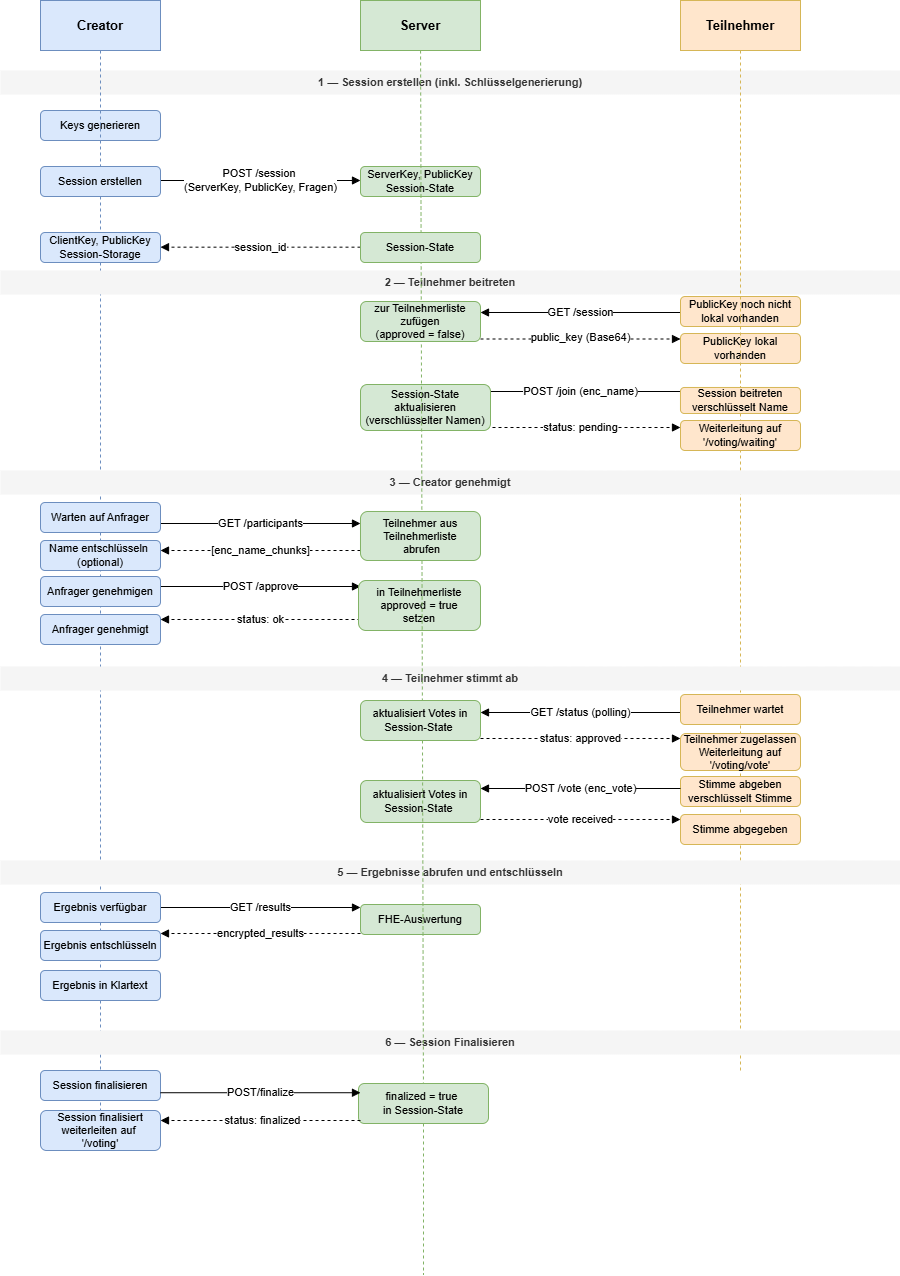
\includegraphics[width=\textwidth]{contents/media/uc32.png}
\end{figure}

\subsubsection{OpenAPI-Schnittstelle}
Der Service stellt eine fachliche Voting-/Polling-API bereit, mit der
Sessions erstellt, Teilnehmer verwaltet und verschlüsselte Stimmen
abgegeben werden können. Die OpenAPI-Definition wird automatisch
generiert und ist unter \texttt{/openapi.json} sowie \texttt{/docs}
(Swagger UI) verfügbar.

Im gesamten Service wird der PublicKey als CompressedPublicKey
verwendet. Dieser ermöglicht eine Batch-Verschlüsselung.

\textbf{POST/session}
Legt eine neue Voting-Session an.


\textbf{Request}:
\begin{lstlisting}
{
  "creator_id": "string",
  "server_key": "string",
  "public_key": "string | null",
  "questions": [
    {
      "id": 0,
      "text": "string",
      "question_type": "single | multiple | numeric",
      "options": ["string"]
    }
  ]
}
\end{lstlisting}

\textbf{Response 200}:
\begin{lstlisting}
{
  { "session_id": "uuid" }
}
\end{lstlisting}

\textbf{Fehlercodes}: 400 – Invalid Base64 oder beschädigtes bincode im server\_key

\textbf{GET /session/{session\_id}
} - Gibt die Metadaten einer Session für Teilnehmer zurück.

\textbf{Response 200}
\begin{lstlisting}
{
  {
      "session_id": "uuid",
      "questions": [
        {
          "id": 0,
          "text": "string",
          "question_type": "single | multiple | numeric",
          "options": ["string"]
        }
      ],
      "public_key": "string | null"
    }
}
\end{lstlisting}
\textbf{Fehlercodes}: 400 – Session nicht gefunden

\textbf{POST/JOIN}
Teilnehmer beantragt den Beitritt zu einer Session. Der Beitritt ist zunächst pending und muss vom Creator freigegeben werden.
\textbf{Response 200}
\begin{lstlisting}
{
  {
      "session_id": "uuid",
      "participant_id": "string",
      "enc_name_chunks": ["string"]
    }
}
\end{lstlisting}


\textbf{Response 200}
\begin{lstlisting}
{
  { "status": "pending" }
}
\end{lstlisting}
\textbf{Fehlercodes}

404 – Session nicht gefunden

409 – Session bereits beendet



\textbf{POST/APPROVE}

Der Creator genehmigt oder lehnt Teilnehmer ab.
\textbf{Request}
\begin{lstlisting}
{
  {
      "session_id": "uuid",
      "creator_id": "string",
      "participant_id": "string",
      "approved": true
    }
}
\end{lstlisting}

\textbf{Response 200}
\begin{lstlisting}
{
  { "status": "ok" }
}
\end{lstlisting}
\textbf{Fehlercodes}

404 – Session nicht gefunden

403 – Nicht autorisiert (falscher creator\_id)

409 – Session bereits beendet

404 – Teilnehmer nicht gefunden (nur bei approval=true relevant)

\textbf{POST /vote}

Ein genehmigter Teilnehmer sendet seine verschlüsselten Votes.
\begin{lstlisting}
{
  {
      "session_id": "uuid",
      "participant_id": "string",
      "encrypted_votes": [
        ["string"],
        ["string"]
      ]
    }
}
\end{lstlisting}

\textbf{Response 200}
\begin{lstlisting}
{
  { "status": "vote received" }}
}
\end{lstlisting}


\textbf{Fehlercodes}

404 – Session nicht gefunden

404 – Teilnehmer nicht gefunden

403 – Teilnehmer nicht genehmigt

409 – Session bereits beendet

400 – Anzahl der Votes stimmt nicht mit Fragen überein


\textbf{GET /status/{session\_id}/{participant\_id}}

Liefert den aktuellen Status eines Teilnehmers.

\textbf{Response 200}
\begin{lstlisting}
{
  [
      {
        "participant_id": "string",
        "approved": true,
        "has_voted": false,
        "enc_name_chunks": ["string"]
      }
    ]
}
\end{lstlisting}


\textbf{Fehlercodes}

404 – Session nicht gefunden

403 – Nicht autorisiert

\textbf{GET /results/{session\_id}/{creator\_id}}
Gibt die homomorph aggregierten Ergebnisse zurück (nur Creator). Wenn noch nicht alle Votes vorhanden sind, ist ready = false.

\textbf{Response (ready)}
\begin{lstlisting}
{
  {
      "encrypted_results": [
        ["string"]
      ],
      "ready": true
    }
}
\end{lstlisting}

 \textbf{Response (not ready)}
\begin{lstlisting}
{
  {
      "encrypted_results": [],
      "ready": false
    }
}
\end{lstlisting}

 \textbf{Fehlercodes}

404 – Session nicht gefunden

403 – Nicht autorisiert


\textbf{POST /finalize/{session\_id}/{creator\_id}}

Schließt die Session endgültig. Danach sind keine Votes oder Joins mehr möglich.

\textbf{Response 200}
\begin{lstlisting}
{
  { "status": "finalized" }
}
\end{lstlisting}

 \textbf{Fehlercodes}

404 – Session nicht gefunden

403 – Nicht autorisiert

409 – Session bereits finalisiert

\subsubsection{Trust- und Threat-Model}

\begin{longtable}{|p{5cm}|c|c|c|}
\hline
\textbf{Datum} &
\textbf{Am Server klar} &
\textbf{Am Server verschlüsselt} &
\textbf{Am Client} \\
\hline
\endfirsthead

\hline
\textbf{Datum} &
\textbf{Am Server klar} &
\textbf{Am Server verschlüsselt} &
\textbf{Am Client} \\
\hline
\endhead

\hline
\endfoot

\hline
\endlastfoot

Session\_id (UUID) & X & & X \\
\hline
Creator\_id & X & & X \\
\hline
Participant\_id & X & & X \\
\hline
Fragen & X & & X \\
\hline
Antwortoptionen & X & & X \\
\hline
Teilnehmerstatus & X & & X \\
\hline
Abstimmungszeitpunkte & X & & X \\
\hline
Anzahl Teilnehmer/Votes & X & & X \\
\hline
Session State (finalized) & X & & X \\
\hline
Public Key der Session & X & & X \\
\hline
Server Key & X & & X \\
\hline
Teilnehmernamen (verschlüsselt) & & X & X \\
\hline
Teilnehmernamen (entschlüsselt) & & & X \\
\hline
Vote Inhalt & & X & \\
\hline
Aggregierte Ergebnisse (verschlüsselt) & & X & X \\
\hline
Aggregierte Ergebnisse (entschlüsselt) & & & X \\
\hline
Client Key & & & X \\
\hline

\caption{Datenhaltung im Voting-Service}
\label{tab:voting-datenhaltung}
\end{longtable}

\textbf{Analyse: Beobachtbare Metadaten}

TFHE schützt ausschließlich die Inhalte von Stimmen und Ergebnissen. Für den Server bleiben weiterhin verschiedene Metadaten sichtbar:

\begin{itemize}
    \item Anzahl und Aktivität von Sessions
    \item Anzahl der Teilnehmer pro Session
    \item Anzahl abgegebener Stimmen
    \item Zeitpunkte von Beitritt, Genehmigung und Abstimmung
    \item Request-Timing und Voting-Pattern
    \item Umfragestruktur (Fragen und Antwortoptionen)
    \item Teilnehmerstatus (pending, approved, has\_voted)
    \item Polling-Verhalten der Admin-Oberfläche
\end{itemize}

Ein Server-Operator kann daraus Rückschlüsse auf Aktivitätsmuster, soziale Dynamiken, die Größe einer Abstimmung oder mögliche Zusammenhänge zwischen Abstimmungszeitpunkten und Teilnehmerverhalten ziehen. 

Der Server kann zwar keine Stimmen entschlüsseln, muss jedoch weiterhin als korrekter Ausführer des Protokolls vertrauenswürdig sein. Insbesondere wird angenommen, dass der Server:

\begin{itemize}
    \item Teilnehmer korrekt Sessions zuordnet
    \item Join- und Approval-Prozesse korrekt verarbeitet
    \item Stimmen vollständig speichert und nicht verwirft
    \item Sessions voneinander trennt
    \item Homomorphe Aggregationen korrekt ausführt
    \item Die Verfügbarkeit des Systems sicherstellt
\end{itemize}

TFHE reduziert somit die Vertrauensabhängigkeit hinsichtlich der Inhaltsvertraulichkeit, ersetzt jedoch kein vollständig vertrauensloses Protokoll.

\textbf{Annahmen außerhalb von TFHE}

Die Sicherheitsbetrachtung basiert auf folgenden Annahmen:

\begin{itemize}
    \item Die Kommunikation zwischen Client und Server erfolgt über TLS.
    \item Das Frontend führt die Verschlüsselung und Entschlüsselung korrekt aus.
    \item Die verwendete TFHE-rs-Bibliothek wird als kryptographisch korrekt implementierte Black Box betrachtet. Der ClientKey verbleibt ausschließlich beim Session-Ersteller.
\end{itemize}

Das System besitzt keine starke Benutzerauthentifizierung, die Teilnahme erfolgt ausschließlich über Session-ID und frei gewählten Namen.

\textbf{Schutzversprechen}

Durch den Einsatz von TFHE wird garantiert:

\begin{itemize}
    \item Der Server kann individuelle Stimmen nicht im Klartext lesen.
    \item Der Server kann einzelne Abstimmungsentscheidungen nicht rekonstruieren.
    \item Stimmen werden ausschließlich verschlüsselt verarbeitet. Auch aggregierte Ergebnisse liegen auf dem Server nur verschlüsselt vor.
\end{itemize}

Nicht garantiert werden:

\begin{itemize}
    \item Vertraulichkeit der Umfragestruktur
    \item Vertraulichkeit von Metadaten und Abstimmungszeitpunkten
    \item Schutz vor Traffic- und Timing-Analysen
    \item Schutz vor aktiv manipulierendem Serververhalten
    \item Fairness oder Vollständigkeit der Protokollausführung
\end{itemize}

Konkret bedeutet das: Der Server kennt nicht den Inhalt einer abgegebenen Stimme und kann nicht feststellen, welche Antwort ein Teilnehmer gewählt hat. Sichtbar bleiben jedoch Existenz, Zeitpunkt und organisatorischer Kontext der Abstimmung.

\textbf{Einordnung}

Der Use Case implementiert ein TFHE-geschütztes Abstimmungssystem mit Vertraulichkeit auf Inhaltsebene. Geschützt werden ausschließlich individuelle Stimmen und deren aggregierte Ergebnisse. Metadaten, Umfragestruktur und der allgemeine Kontrollfluss der Anwendung bleiben außerhalb des Schutzbereichs von TFHE.

\subsubsection{FHE-Designentscheidungen}

\textbf{Verwendete TFHE-rs-Typen}

Für die Repräsentation der Stimmen wird primär der Datentyp FheUint32 verwendet. Obwohl die einzelnen Eingabewerte der Teilnehmer (z. B. bei numerischen Fragen oder kodierten Auswahlwerten) nur im Bereich 0 kleiner gleich x kleiner gleich 255 liegen und damit grundsätzlich mit FheUint8 darstellbar wären, wurde bewusst ein größerer Datentyp gewählt.

Der Grund liegt in der homomorphen Aggregation der Stimmen. Alle Einzelwerte werden serverseitig addiert, wodurch das Ergebnis deutlich größere Werte annehmen kann als der ursprüngliche Eingabebereich. Bei k Teilnehmern ergibt sich im Worst Case: 255 x k

Um Überläufe sicher auszuschließen und eine einheitliche Verarbeitung aller Fragetypen zu gewährleisten, wird daher FheUint32 sowohl für Einzelstimmen als auch für aggregierte Ergebnisse verwendet. Dies vereinfacht zusätzlich die Implementierung, da kein Typwechsel zwischen Eingabe und Auswertung erforderlich ist.

Für Teilnehmernamen wird dagegen FheUint8 verwendet. Jeder Buchstabe wird als ASCII-Zeichenwert (0–255) verschlüsselt und einzeln gespeichert. Da Zeichenwerte innerhalb dieses Bereichs liegen, ist ein größerer Datentyp hierfür nicht erforderlich.

\textbf{Verwendete homomorphe Operationen}

Der Server führt ausschließlich homomorphe Additionen auf verschlüsselten Stimmen aus. Für jede Frage werden die verschlüsselten Stimmen aller Teilnehmer aufsummiert. Bei Single-Choice- und Multiple-Choice-Fragen erfolgt die Addition komponentenweise für jede Antwortoption. Andere homomorphe Operationen werden nicht benötigt, dadurch bleibt die serverseitige Auswertung auf die einfachste benötigte FHE-Operation beschränkt.

\textbf{Verworfene Alternativen}

Separate Bool-Fragen (FheBool)

Ursprünglich war vorgesehen, Ja/Nein-Fragen als eigene Kategorie abzubilden. Diese Variante wurde verworfen. Stattdessen können Ja/Nein-Fragen als Single-Choice-Fragen mit den Antwortoptionen „Ja“ und „Nein“ modelliert werden.

Dadurch müssen alle Fragen zwingend beantwortet werden und die Auswertung aller Auswahlfragen kann über denselben Algorithmus erfolgen. Zudem entfällt die Notwendigkeit, unterschiedliche verschlüsselte Datentypen (FheBool und FheUint32) parallel zu unterstützen. Die Implementierung verwendet somit ausschließlich FheUint32 für die Repräsentation von Stimmen.

FheUint8 als Speichertyp für Stimmen

FheUint8 wäre für einzelne Stimmen semantisch korrekt, da Eingabewerte auf 0–255 begrenzt sind. Dieser Ansatz wurde jedoch verworfen, da die homomorphe Aggregation schnell zu Überläufen führen würde.

Stattdessen wird einheitlich FheUint32 verwendet, um sowohl Einzelwerte als auch Summen sicher darzustellen.

Gleitkommazahlen

Gleitkommazahlen wurden als naheliegende Repräsentation für numerische Eingaben verworfen, da TFHE primär auf Ganzzahlarithmetik ausgelegt ist. Insbesondere Divisionen und Floating-Point-Operationen sind entweder nicht vorgesehen oder ineffizient. Daher erfolgt die Modellierung aller Werte als Ganzzahlen (FheUint32).

\subsubsection{Komplexität der eigenen Algorithmen}

\begin{itemize}
    \item n: Anzahl der Fragen einer Abstimmung
    \item k: Anzahl der Teilnehmer bzw. abgegebenen Stimmen
    \item m: Anzahl der Antwortoptionen einer Single- oder Multiple-Choice-Frage
\end{itemize}
Die interne Komplexität der TFHE-rs-Bibliothek wird nicht betrachtet; jede homomorphe Operation wird gemäß Aufgabenstellung als O(1) angenommen.

\begin{table}[h]
\centering
\begin{tabular}{|l|c|c|}
\hline
\textbf{Funktion} & \textbf{Zeitkomplexität} & \textbf{Platzkomplexität} \\
\hline
create\_session & $O(n)$ & $O(n)$ \\
\hline
join\_session & $O(1)$ & $O(1)$ \\
\hline
approve\_participant & $O(1)$ & $O(1)$ \\
\hline
submit\_vote & $O(nm)$ & $O(nm)$ \\
\hline
aggregate\_votes\_ciphertext\_only & $O(nkm)$ & $O(m)$ \\
\hline
get\_results & $O(k + nkm)$ & $O(nkm)$ \\
\hline
finalize\_session & $O(1)$ & $O(1)$ \\
\hline
get\_status & $O(1)$ & $O(1)$ \\
\hline
get\_session & $O(n)$ & $O(n)$ \\
\hline
get\_participants & $O(k)$ & $O(k)$ \\
\hline
\end{tabular}
\caption{Big-O-Komplexitäten des Encrypted-Voting-Service}
\label{tab:voting-komplexitaet}
\end{table}

Create\_session -- $O(n)$, $O(n)$

Beim Anlegen einer Session wird die übergebene Fragenliste gespeichert. Die übrigen Operationen (UUID-Erzeugung, Initialisierung leerer HashMaps, Einfügen in die Session-Map) besitzen konstante Laufzeit. Da die Größe der Fragenliste proportional zu n ist, ergeben sich Zeit- und Platzkomplexität von O(n).

Join\_session -- $O(1)$, $O(1)$

Die Session wird per HashMap-Lookup gefunden und ein neuer Teilnehmer in die Teilnehmer-HashMap eingefügt. Beide Operationen besitzen durchschnittlich konstante Laufzeit. Pro Aufruf wird nur ein zusätzlicher Teilnehmer gespeichert.

Approve\_participant –- $O(1)$, $O(1)$

Die Session und der Teilnehmer werden über HashMaps gefunden. Anschließend wird entweder ein Boolean gesetzt oder der Teilnehmer entfernt. Es erfolgt keine Iteration über Teilnehmer oder Stimmen.

Submit\_vote -– $O(nm)$, $O(nm)$

Eine Stimme enthält für jede der n Fragen verschlüsselte Antworten. Bei Single-/Multiple-Choice-Fragen können pro Frage bis zu m verschlüsselte Optionen enthalten sein. Das Speichern der gesamten Stimmenstruktur benötigt daher Zeit und Speicher proportional zur Anzahl der übergebenen verschlüsselten Werte.

Aggregate\_votes\_ciphertext\_only -– $O(nkm)$, $O(m)$

Für jede der $n$ Fragen werden alle $k$ Stimmen verarbeitet. Bei Single- oder Multiple-Choice-Fragen werden zusätzlich alle $m$ Antwortoptionen aufsummiert. Daraus ergibt sich eine Zeitkomplexität von $O(n \cdot k \cdot m)$.

Der zusätzliche Speicher besteht lediglich aus dem Akkumulatorvektor für die aktuelle Frage und benötigt maximal m Einträge.

Get\_results -– $O(k+nkm)$, $O(nkm)$

Zunächst werden alle Teilnehmer durchlaufen, um die Anzahl der freigegebenen Teilnehmer zu bestimmen (O(k)). Anschließend werden alle gespeicherten Stimmen kopiert und aggregiert. Die Aggregation dominiert mit $O(nkm)$. Für die Kopie aller Stimmen wird Speicher proportional zur Gesamtzahl gespeicherter Stimmen benötigt: $O(nkm)$

Finalize\_session -– $O(1)$, $O(1)$

Die Session wird per HashMap gefunden und das Boolean-Feld finalized gesetzt. Es werden weder Schleifen noch zusätzliche Datenstrukturen verwendet.

Get\_status -– $O(1)$, $O(1)$

Der Teilnehmerstatus wird über einen einzelnen HashMap-Zugriff bestimmt. Es erfolgt keine Iteration über andere Teilnehmer.

Get\_session –- $O(n)$, $O(n)$

Die Session wird per HashMap gefunden und die Fragenliste in die Antwort kopiert. Die Größe dieser Liste ist proportional zur Anzahl der Fragen n.

Get\_participants -– $O(k)$, $O(k)$

Für die Antwort wird über alle Teilnehmer iteriert und für jeden ein ParticipantAdminView erzeugt. Jeder Teilnehmer wird genau einmal verarbeitet, daher ergibt sich eine lineare Laufzeit und Speicherbelegung in der Anzahl der Teilnehmer k.

\subsubsection{Performance-Messung}

Mess-Setup \& Methodik

Die Performance- und Stresstests wurden auf einem virtuellen KVM-Server von Netcup mit dedizierten CPU-Ressourcen durchgeführt. Die Last wurde extern mittels k6 von einer lokalen Windows-Maschine über das Internet injiziert.

Es wurden zwei Testszenarien mit unterschiedlichen funktionalen Schwerpunkten untersucht:

\begin{itemize}
    \item Teilnehmer-Anfragen: Analyse der Endpunkte (POST /join und GET /status), um das Systemverhalten bei einem Anstieg von Join-Anfragen und hochfrequentem Polling durch die Teilnehmer zu evaluieren.
    \item \item Ergebnisauswertung: Dedizierte Stressprüfung des Endpunkts \texttt{GET /results/\{session\_id\}/\{creator\_id\}} unter einer Dauerlast von konstant zehn parallelen Virtual Users (VUs). Um die CPU-Auslastung durch die kryptografischen Berechnungen gezielt zu maximieren, wurde das System vorab in einen Zustand versetzt, in dem die Bedingung \texttt{voted\_count >= approved\_count} dauerhaft erfüllt war. Dadurch wurde sichergestellt, dass jeder eingehende Request die rechenintensive homomorphe Aggregationsfunktion \texttt{aggregate\_votes\_ciphertext\_only} vollständig durchläuft. Das Szenario wurde in zwei separaten Testläufen durchgeführt: zunächst mit zwei Teilnehmern und anschließend mit zehn Teilnehmern pro Session.
\end{itemize}

Performancetest 1 (Join und Polling) (08.06.2026)

Im ersten Testszenario wurde ein plötzlicher Anstieg der Teilnehmeraktivität simuliert. Die Anzahl der virtuellen Nutzer wurde innerhalb von zwei Sekunden von fünf auf 500 erhöht. Jeder Teilnehmer führte genau eine Join-Anfrage aus und wechselte anschließend in ein hochfrequentes Polling des Sitzungsstatus mit einem Intervall von 200 ms.

\begin{table}[h]
\centering
\begin{tabular}{|l|c|c|}
\hline
\textbf{Metrik} & \textbf{join} & \textbf{status} \\
\hline
p50 & 17,48 ms & 17,16 ms \\
\hline
p90 & 21,92 ms & 21,32 ms \\
\hline
p95 & 24,45 ms & 25,02 ms \\
\hline
Maximum & 41,86 ms & 95,06 ms \\
\hline
Fehlerrate & 0\,\% & 0\,\% \\
\hline
\end{tabular}
\caption{Latenzkennzahlen der Endpunkte \texttt{join} und \texttt{status}}
\label{tab:join-status-metriken}
\end{table}

Fazit von Performancetest 1:

Während des gesamten Tests wurden insgesamt 105.675 HTTP-Anfragen verarbeitet. Dabei konnten keine fehlgeschlagenen Requests beobachtet werden. Sowohl die Join- als auch die Status-Endpunkte zeigten stabile Antwortzeiten im niedrigen zweistelligen Millisekundenbereich (Join: p95 = 24,45 ms; Status: p95 = 25,02 ms), sodass im untersuchten Lastbereich keine Hinweise auf Engpässe oder Skalierungsprobleme festgestellt werden konnten.

Performancetest 2: FHE-Ergebnisauswertung (03.06.2026)

Hierbei wurde die mathematisch rechenintensive homomorphe Aggregation evaluiert. Um den direkten Einfluss der Kryptographischen Komplexität zu untersuchen, wurde derselbe Stresstest bei dauerhaft 10 parallelen VUs in zwei getrennten Konfigurationen durchgeführt, einmal mit 2 hinterlegten Stimmen und einmal mit 10 hinterlegten Stimmen. Die Auswahl von genau 2 bzw. 10 Teilnehmern erfolgte, um einerseits die mathematische Grundlatenz zu bestimmen und andererseits die Skalierung der FHE-Operation unter moderater Gruppenlast zu überprüfen.

\begin{table}[h]
\centering
\begin{tabular}{|l|c|c|}
\hline
\textbf{Metrik} & \textbf{2 Stimmen} & \textbf{10 Stimmen} \\
\hline
p50 & 0,47 s & 2,83 s \\
\hline
p90 & 0,51 s & 8,31 s \\
\hline
p95 & 0,53 s & 11,21 s \\
\hline
Maximum & 0,76 s & 14,32 s \\
\hline
Fehlerrate & 0\,\% & 0\,\% \\
\hline
Durchsatz & 1,49 Request/s & 0,90 Request/s \\
\hline
\end{tabular}
\caption{Ergebnisse des zweiten Stresstests für die Ergebnisauswertung mit zwei bzw. zehn Stimmen}
\label{tab:stresstest-ergebnisse}
\end{table}

Während das System bei 2 Stimmen sehr schnell reagiert, führt die rechenintensive kryptografische Funktion aggregate\_votes\_ciphertext\_only bei 10 Stimmen zu einer massiven Latenz von über 11 Sekunden im p95-Bereich. Diese Verzögerung resultiert aus der globalen Zustandssperre $(state.lock())$. Da dieser Mutex während der gesamten FHE-Berechnung gehalten wird, blockiert er die parallele Verarbeitung des Axum-Servers und führt zu einer sequenziellen Abarbeitung aller eingehenden Anfragen. Trotz dieser intensiven CPU-Auslastung arbeitet das Backend vollständig stabil und verarbeitet alle Anfragen ohne Fehlerraten.


\begin{figure}[H]
    \centering
    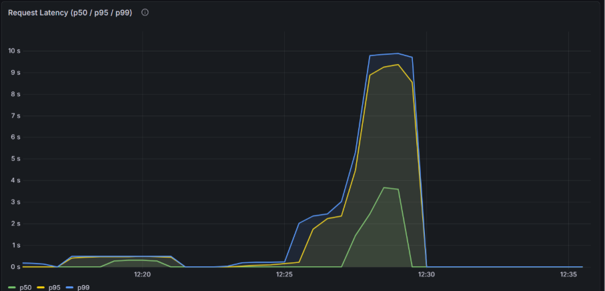
\includegraphics[width=\textwidth]{contents/media/uc31.png}
\end{figure}

n der Grafik findet sich die Testvariante mit 2 hinterlegten Stimmen im Bereich von ca. 12:17–12:22. Hier wird sichtbar, dass das System sehr schnell reagiert und p95 und p99 nahezu identisch verlaufen.

Die Variante mit 10 hinterlegten Teilnehmern findet sich im Bereich von ca. 12:26–12:30. Hier zeigt sich ein drastischer Umschwung im Systemverhalten: Die Latenzkurven für p95 und p99 brechen steil nach oben aus und bilden ein massives Plateau, das sich knapp unterhalb der 10-Sekunden-Marke einpendelt. Die grüne Median-Linie (p50) verläuft deutlich darunter im Bereich von knapp 3 Sekunden, was die Verteilung der Wartezeiten im eingetretenen Mutex-Stau exakt widerspiegelt. Der absolute Peak von 14,32 Sekunden wird kurz vor dem Ende des Testfensters als dünne, maximale Spitze der blauen p99-Kurve sichtbar. Nach dem harten Stopp der Last um Punkt 12:30 Uhr fällt die Latenz sofort wieder auf die Baseline von 0 Sekunden ab.

Zusammenfassend zeigen die Messergebnisse, dass die grundlegende REST-Infrastruktur des Backends (Test 1) optimal skaliert und im unverschlüsselten Zustand keinerlei Performance-Engpässe aufweist. Die eigentliche Skalierungsbremse des Systems liegt isoliert auf der kryptographischen Verarbeitungsebene (Test 2).

\subsubsection{Limitationen}

\begin{itemize}
    \item Teilnehmende können bei numerischen Fragen ausschließlich Werte zwischen 0 und 255 als Antwort angeben. Höhere Zahlen lassen wir bewusst nicht zu, demenstprechend müssen Fragen eventuell anders definiert werden. Bsp: Wie hoch ist dein Jahregehalt in tausend €
    \item Es können keine Doppelabstimmungen verhindert werden. Ein Teilnehmer kann technisch mehrere Join-Requests mit unterschiedlichen Namen schicken und so mehrfach abstimmen. Stattdessen erfolgt die Kontrolle durch den Ersteller. Dadurch liegt die Verantwortung für die Verhinderung von Mehrfachteilnahmen bei ihm.
\end{itemize}